%\documentclass[mathserif]{beamer}
\documentclass[handout]{beamer}
%\usetheme{Goettingen}
\usetheme{Warsaw}
%\usetheme{Singapore}
%\usetheme{Frankfurt}
%\usetheme{Copenhagen}
%\usetheme{Szeged}
%\usetheme{Montpellier}
%\usetheme{CambridgeUS}
%\usecolortheme{}
%\setbeamercovered{transparent}
\usepackage[english, activeacute]{babel}
\usepackage[utf8]{inputenc}
\usepackage{amsmath, amssymb}
\usepackage{dsfont}
\usepackage{graphics}
\usepackage{cases}
\usepackage{graphicx}
\usepackage{pgf}
\usepackage{epsfig}
\usepackage{amssymb}
\usepackage{multirow}	
\usepackage{amstext}
\usepackage[ruled,vlined,lined]{algorithm2e}
\usepackage{amsmath}
\usepackage{epic}
\usepackage{epsfig}
\usepackage{fontenc}
\usepackage{framed,color}
\usepackage{palatino, url, multicol}
\usepackage{listings}
%\algsetup{indent=2em}


\vspace{-0.5cm}
\title{Introduction to Reinforcement Learning}
\vspace{-0.5cm}
\author[Felipe Bravo Márquez]{\footnotesize
%\author{\footnotesize  
 \textcolor[rgb]{0.00,0.00,1.00}{Felipe José Bravo Márquez}} 
\date{ \today }




\begin{document}
\begin{frame}
\titlepage


\end{frame}


%%%%%%%%%%%%%%%%%%%%%%%%%%%


\begin{frame}{Markov Decision Process}
\scriptsize{
\begin{itemize}
\item A markov decision process is a tuple: 
\begin{displaymath}
 (S,A,\{P_{SA}\},\gamma,R)
\end{displaymath}
where
\item $S$ is a set os states.
\item $A$ is a set of actions.
\item $P_{SA}$ are the state transition probabilites:

\begin{displaymath}
 \sum_{s'}P_{SA}(s')=1, \quad P_{SA}(s')\geq 0
\end{displaymath}

\item $\gamma \in [0,1)$ is a discount factor.

\item $R$ is a reward function.$R: S \rightarrow \mathcal{R}$.

\end{itemize}


} 

\end{frame}



\begin{frame}{Example}
\scriptsize{
\begin{itemize}
\item Suppose that an agent is situated in the $4\times 3$ environment shown in the Figure 


  \begin{figure}[h]
        	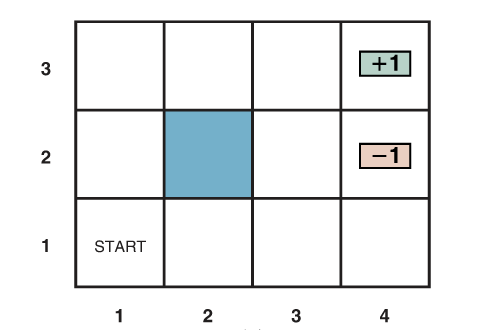
\includegraphics[scale = 0.4]{pics/example.png}
        \end{figure}

\item Beginning in the start state, it must choose an action at each time step. 

\item The interaction with the environment terminates when the agent reaches one of the goal states, marked +1 or –1.

\end{itemize}


} 

\end{frame}


\begin{frame}{Example}
\scriptsize{
\begin{itemize}
\item The ``intended'' outcome occurs with probability 0.8, but with probability 0.2 the agent moves at right angles to the intended direction:

  \begin{figure}[h]
        	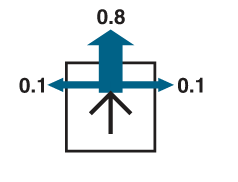
\includegraphics[scale = 0.4]{pics/example1.png}
        \end{figure}

\item A collision with a wall results in no movement.

\item Transitions into the two terminal states have reward +1 and –1, respectively.

\item All other transitions have a reward of –0.02 (to avoid the robot wasting time).
\end{itemize}


} 

\end{frame}

%%%%%%%%%%%%%%%%%%%%%%%%%%%
\begin{frame}[allowframebreaks]\scriptsize
\frametitle{References}
\bibliography{bio}
\bibliographystyle{apalike}
%\bibliographystyle{flexbib}
\end{frame}  









%%%%%%%%%%%%%%%%%%%%%%%%%%%

\end{document}
